\documentclass[conference]{IEEEtran}
\IEEEoverridecommandlockouts

\usepackage{cite}
\usepackage{amsmath,amssymb,amsfonts}
\usepackage{algorithmic}
\usepackage{graphicx}
\usepackage{textcomp}
\usepackage{xcolor}
\usepackage{booktabs}
\usepackage{multirow}
\usepackage{siunitx}
\usepackage{float}
\usepackage[caption=false,font=footnotesize]{subfig}
\usepackage{hyperref}

\newcommand{\acDRL}{deep reinforcement learning (DRL)}
\newcommand{\acHVAC}{heating, ventilation, and air conditioning (HVAC)}
\newcommand{\acRL}{reinforcement learning (RL)}
\newcommand{\acMDP}{Markov decision process (MDP)}
\newcommand{\acOOD}{out-of-distribution (OOD)}
\newcommand{\acCOP}{coefficient of performance (COP)}
\newcommand{\acGHI}{global horizontal irradiance (GHI)}
\newcommand{\acMAE}{mean absolute error (MAE)}
\newcommand{\acRMSE}{root mean square error (RMSE)}
\newcommand{\acDR}{domain randomization (DR)}
\newcommand{\acSB}{Stable-Baselines3 (SB3)}

\graphicspath{{figures/}{plots/}}

\title{DRL-Based HVAC Control for a Single-Zone Smart Building:\\%
A Comparative Study of Control Agents%
\thanks{Final Report submitted for ML709: IoT Smart Systems, Services,
and Applications. Instructor: Prof.~Mohsen Guizani, Mohamed Bin Zayed
University of Artificial Intelligence.}}

\author{%
  \IEEEauthorblockN{%
    Saif Alkindi\IEEEauthorrefmark{1},~%
    Hamdan Alhadhrami\IEEEauthorrefmark{1},~%
    Khalfan Hableel\IEEEauthorrefmark{1}~and~%
    Ali Alharthi\IEEEauthorrefmark{1}%
  }
  \IEEEauthorblockA{%
    \IEEEauthorrefmark{1}Mohamed Bin Zayed University of Artificial Intelligence\\%
    Student IDs: 25011027,~25010875,~25011026,~22010335%
  }%
}

\begin{document}

\maketitle

\begin{abstract}
Buildings account for a large share of global energy use, and HVAC is one of their largest controllable loads. This paper studies deep reinforcement learning for continuous HVAC control in a single-zone smart building and compares PPO, A2C, SAC, and TD3 against a tuned PID baseline. The environment combines nonlinear heat transfer, a Carnot-based coefficient of performance, monthly electricity tariffs, domain randomization, and balanced seasonal sampling. Agents are trained on Syracuse weather and evaluated on held-out Albany weather to assess geographic generalization. Over 100 evaluation episodes, TD3 achieves the best median performance with \SI{0.12}{\degreeCelsius} MAE, \SI{16.9}{\kilo\watt\hour\per day} daily energy use, and $99.7\%$ of time within $\pm\SI{0.5}{\degreeCelsius}$ of the setpoint. A2C and SAC also generalize, while PPO trails the other DRL agents. All four DRL methods outperform PID, which achieves \SI{1.01}{\degreeCelsius} median MAE and $63.2\%$ comfort. A lightweight simulator paired with seasonal diversity and parameter uncertainty during training supports transfer to unseen weather.
\end{abstract}

\begin{IEEEkeywords}
Deep reinforcement learning, HVAC control, smart buildings, energy efficiency,
PPO, SAC, TD3, A2C, PID, domain randomization
\end{IEEEkeywords}

\section{Introduction}
\label{sec:introduction}

Buildings are among the largest energy consumers worldwide, and \acHVAC{}
is a major share of that demand. HVAC control is hard because outdoor
temperature, solar gains, wind speed, and electricity prices vary over
time, and building envelopes differ across sites.

Traditional strategies include rule-based control, proportional integral
derivative (PID) control, and model predictive control (MPC). MPC plans
ahead but depends on accurate models, calibrated parameters, and reliable
forecasts, which makes deployment costly. \acDRL{} learns a policy that
maps observations directly to actions, without solving an optimization
problem at every timestep. The open question is generalization: a
controller trained in one climate or simulator may degrade when
deployment conditions change.

We study this problem in a compact setting. A single-zone thermal model
with nonlinear conductance, solar gains, a \acCOP-aware energy term, and
monthly electricity prices is used to compare four continuous-control DRL
agents (PPO, A2C, SAC, TD3) against a tuned PID baseline. Training uses
Syracuse weather only and evaluation uses Albany weather only, giving a
geographic \acOOD{} split. Training also uses domain randomization over
thermal parameters and round-robin seasonal sampling.

The contributions are: (i) a controlled comparison of four DRL agents and
PID under the same task, observation, action, and reward; (ii)
generalization measured by a city-level train/test split; and (iii)
evidence that a lightweight simulator with domain randomization and
balanced seasonal exposure produces policies that transfer to unseen
weather.

\begin{figure*}[!t]
\centering
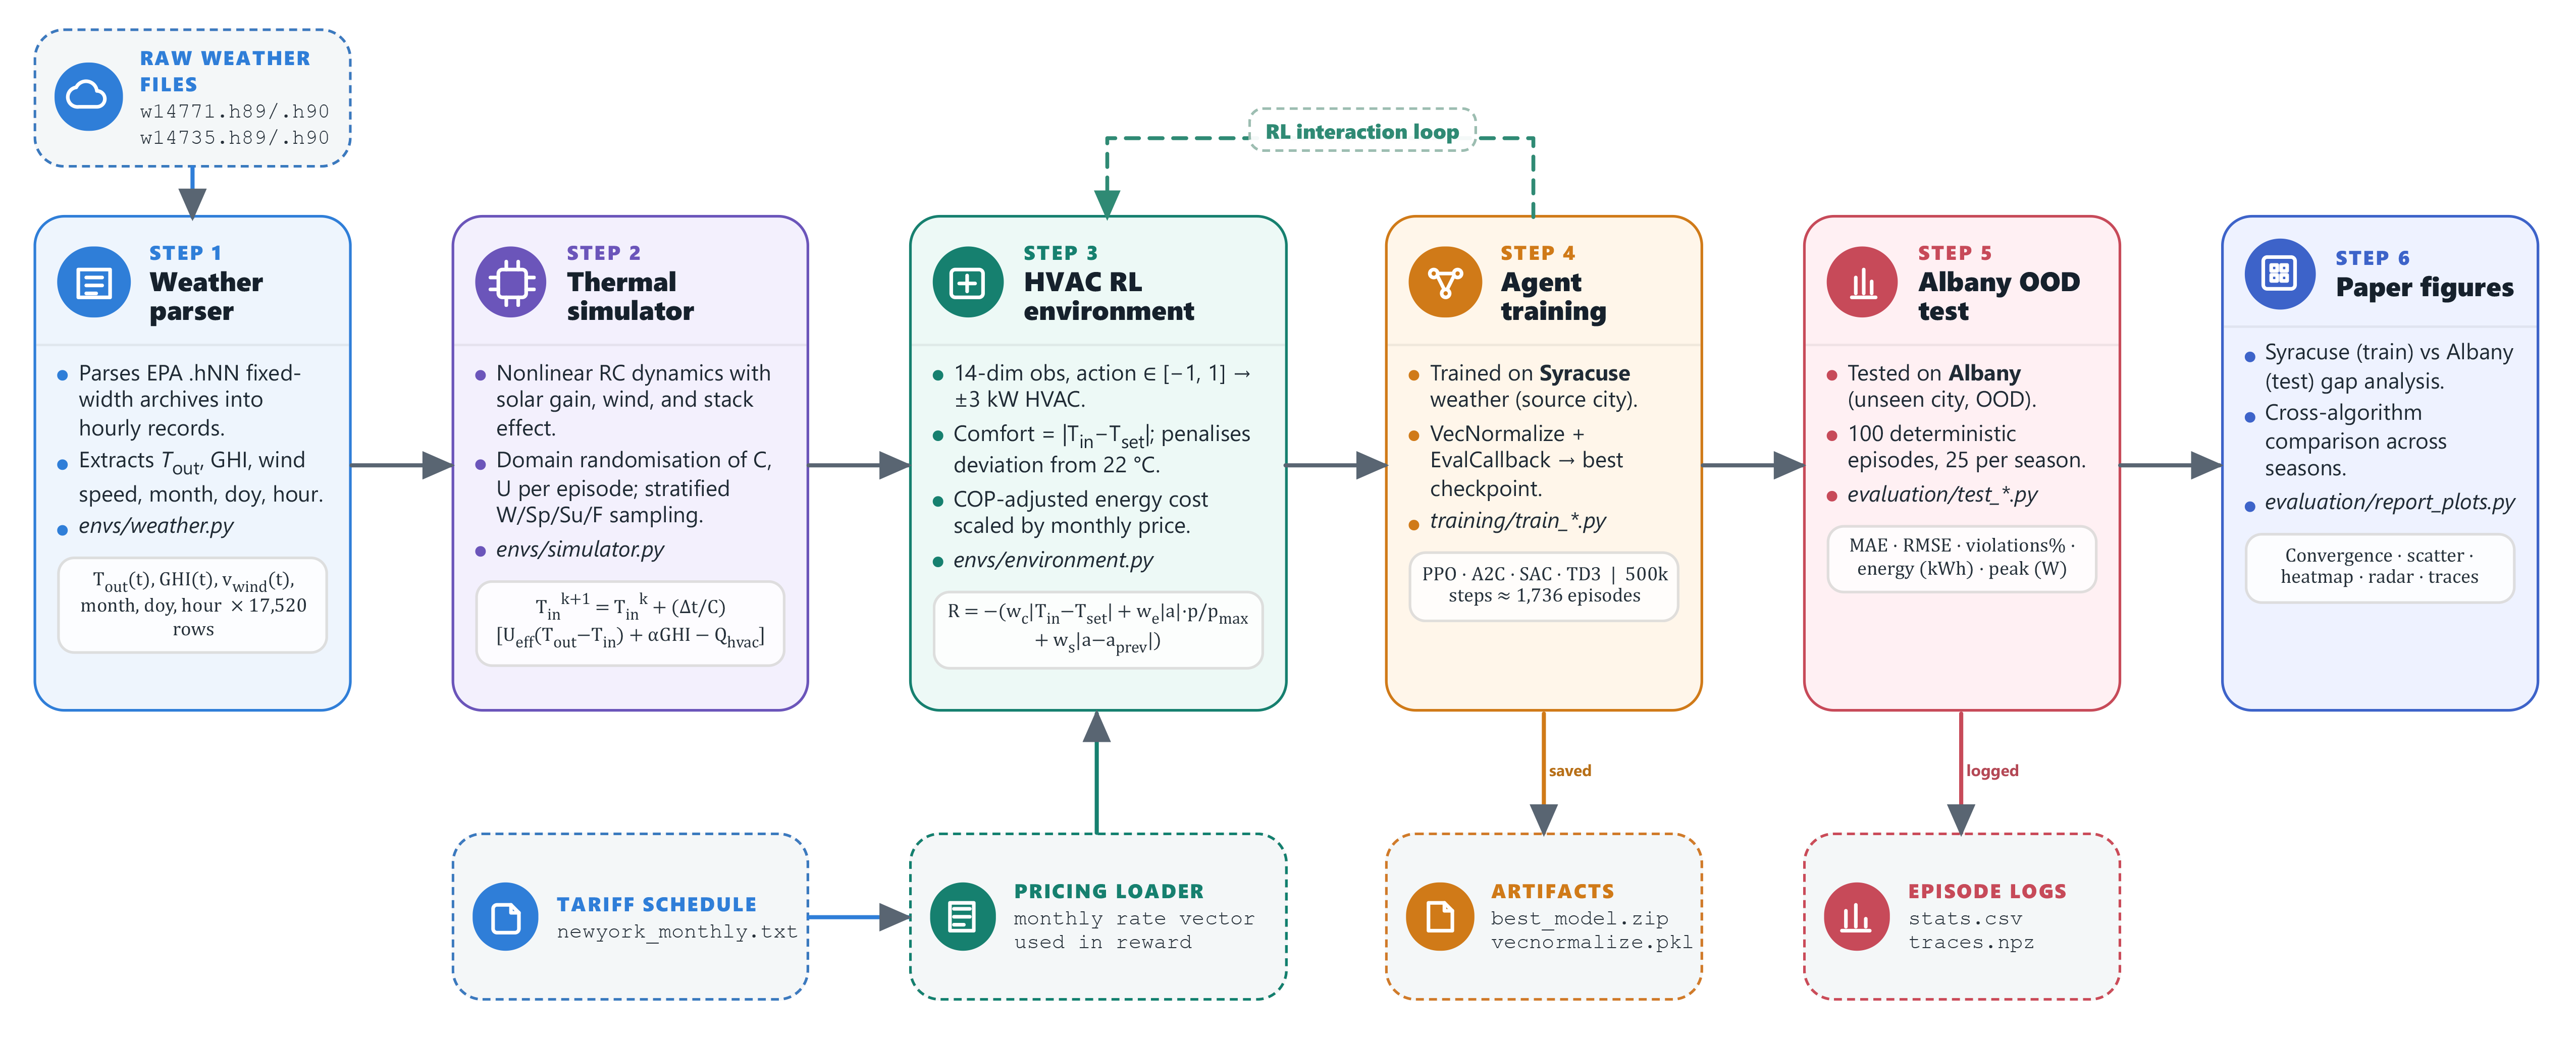
\includegraphics[width=\textwidth]{pipeline.png}
\caption{End-to-end workflow. EPA weather archives and NY electricity tariffs
drive a nonlinear lumped-capacitance simulator with domain randomization and
stratified seasonal sampling, exposed as a 14-dimensional Gymnasium
environment. PPO, A2C, SAC, and TD3 are trained for 500\,k steps on Syracuse
and evaluated out-of-distribution on Albany over 100 episodes (25 per season).}
\label{fig:pipeline}
\end{figure*}

\section{Related Work}
\label{sec:related-work}

Recent surveys report that \acDRL{} can match or exceed MPC on
comfort-energy trade-offs while raising open issues in reward design,
reproducibility, and sensitivity to changing conditions
\cite{manjavacas2024drl_hvac,bekal2025continual_hvac,yu2025rl_urban_hvac}.

For continuous control, A2C/A3C introduced asynchronous advantage
estimation \cite{mnih2016a2c}. PPO replaced trust-region updates with a
clipped surrogate objective and is now a common on-policy baseline
\cite{schulman2017ppo}. TD3 reduced value overestimation through clipped
double critics, delayed policy updates, and target policy smoothing
\cite{fujimoto2018td3}. SAC added maximum-entropy learning with a
stochastic actor and good sample efficiency \cite{haarnoja2018sac}.

The Sinergym benchmark \cite{manjavacas2024drl_hvac} evaluated PPO, TD3,
and SAC across buildings and climates and found that off-policy methods
often produce better trade-offs, while noting that many HVAC papers
compare only one or two algorithms in a single setting. On the transfer
side, a continual DRL study \cite{bekal2025continual_hvac} reported that
transfer and sample efficiency remain bottlenecks, and a model-based SAC
framework with hypernetworks improved transfer and reduced catastrophic
forgetting. Coupling DRL HVAC control with an urban climate model
\cite{yu2025rl_urban_hvac} showed that background climate shifts both
the reward trade-off and policy transferability across cities.

Our work is closest to \cite{manjavacas2024drl_hvac} but targets a
different gap: a simpler single-zone setting that isolates algorithmic
differences, a strict city-level transfer split, and a cost-aware reward
that depends on both electricity price and instantaneous COP.

\section{Environment Design}
\label{sec:environment}

Figure~\ref{fig:pipeline} summarizes the full workflow. Raw weather and
tariff data are parsed into hourly exogenous inputs, which drive a
five-minute physics-based simulator exposed as a Gymnasium environment.
This section describes the data pipeline, the thermal model, and the
episode design choices used to improve generalization.

\subsection{Weather and Tariff Inputs}
\label{subsec:data}

We use U.S.\ Environmental Protection Agency (EPA) PRZM-format hourly
weather archives from 1989 to 1990 for two upstate New York stations:
Syracuse (station 14771), used for training only, and Albany (station
14735), used for evaluation only. Each station contributes about
17\,520 hourly records of outdoor temperature, \acGHI{}, and wind speed.
The split is geographic and enforced at the file-path level in the
codebase, so Albany is never used during training, hyperparameter tuning,
or model selection.

The PRZM \texttt{.hNN} files are fixed-width ASCII tables. A custom parser
extracts the date (cols.\ 2--11, \texttt{yyyy-mm-dd}), the EPA hour index
(cols.\ 12--14, where 1 maps to 00:00 and 25 is a daily summary row that
is discarded), \acGHI{} in \si{\watt\hour\per\metre\squared}
(cols.\ 30--34), dry-bulb outdoor temperature in \si{\degreeCelsius}
(cols.\ 65--69), and wind speed at \SI{10}{\metre} in
\si{\metre\per\second} (cols.\ 96--100). Trailing quality-flag characters
are stripped. Missing values, encoded as \texttt{---}, are forward-filled
and then back-filled to remove short gaps. Small negative \acGHI{} and
wind values caused by rounding artifacts are clipped to zero. The annual
files for each station are then concatenated and sorted into a single
hourly DataFrame with columns \texttt{T\_out}, \texttt{GHI},
\texttt{wind\_speed}, \texttt{month}, \texttt{doy}, and
\texttt{hour\_of\_day}.

Electricity prices are taken from the NYSERDA monthly average residential
retail rate table for New York State. The loader extracts a 12-element
NumPy vector $p \in \mathbb{R}^{12}$ in cents per
\si{\kilo\watt\hour}, indexed by calendar month. During simulation,
each five-minute control step uses a zero-order hold on the most recent
hourly weather row, so the same $T_{\text{out}}$, \acGHI{}, and
$v_{\text{wind}}$ values are applied for twelve consecutive simulator
steps. The month field is used to look up
$p_t = p[\text{month}-1]$, which is exposed to the agent in normalized
form and also used in the reward.


\begin{table}[!t]
\centering
\caption{Thermal Simulator Parameters}
\label{tab:params}
\sisetup{per-mode=symbol}
\begin{tabular}{llc}
\toprule
\textbf{Symbol} & \textbf{Description} & \textbf{Value / Range} \\
\midrule
$C$                 & Thermal capacitance      & $\mathcal{U}$(200\,k, 500\,k)\,\si{\joule\per\degreeCelsius} \\
$U_{\text{cond}}$   & Conduction coefficient   & $\mathcal{U}$(30, 80)\,\si{\watt\per\degreeCelsius} \\
$k_w$               & Wind infiltration coeff. & \SI{4.45}{\watt\per\degreeCelsius} \\
$n_w$               & Wind power-law exponent  & 0.65 \\
$k_s$               & Stack-effect coefficient & \SI{2.6}{\watt\per\degreeCelsius} \\
$\alpha$            & Solar gain coefficient   & \SI{0.5}{\metre\squared} \\
$\eta_{\text{COP}}$ & Carnot efficiency factor & 0.4 \\
$Q_{\max}$          & Maximum HVAC power       & \SI{3000}{\watt} \\
$T_{\text{set}}$    & Temperature setpoint     & \SI{22}{\degreeCelsius} \\
$\Delta t$          & Control timestep         & \SI{300}{\second} \\
\bottomrule
\end{tabular}
\end{table}

\begin{table*}[!t]
\centering
\small
\caption{Observation Space (14-dimensional state vector).}
\label{tab:obs}
\sisetup{per-mode=symbol}
\begin{tabular}{cllll}
\toprule
\textbf{\#} & \textbf{Feature} & \textbf{Range} & \textbf{Group} & \textbf{Description} \\
\midrule
0  & $T_{\text{in}} - T_{\text{set}}$ & $[-50,50]$\,\si{\degreeCelsius} & Thermal   & Indoor temperature error \\
1  & $(T_{\text{out}}-20)/20$         & $[-2,2]$                        & Thermal   & Outdoor temperature, centered and scaled \\
2  & $\sin(2\pi h/24)$                & $[-1,1]$                        & Time      & Hour sine encoding \\
3  & $\cos(2\pi h/24)$                & $[-1,1]$                        & Time      & Hour cosine encoding \\
4  & $\sin(2\pi d/365)$               & $[-1,1]$                        & Time      & Day sine encoding \\
5  & $\cos(2\pi d/365)$               & $[-1,1]$                        & Time      & Day cosine encoding \\
6  & $p_t / p_{\max}$                 & $[0,1]$                         & Exogenous & Price normalized by annual maximum \\
7  & GHI$/1200$                       & $[0,1]$                         & Exogenous & Solar irradiance normalized by 1200 \\
8  & $v_{\text{wind}}/20$             & $[0,1]$                         & Exogenous & Wind speed normalized by 20 \\
9  & $C / C_{\text{nom}}$             & $[0.57,1.43]$                   & DR        & Capacitance ratio \\
10 & $U_{\text{cond}} / U_{\text{cond,nom}}$ & $[0.55,1.45]$               & DR        & Conduction-coefficient ratio \\
11 & $a_{t-1}$                        & $[-1,1]$                        & Actuator  & Previous action \\
12 & COP$/10$                         & $[0.08,1]$                      & Physics   & COP normalized by 10 \\
13 & $U_{\text{eff}}/150$             & $[0,1]$                         & Physics   & Effective conductance normalized by 150 \\
\bottomrule
\end{tabular}
\end{table*}



\subsection{Thermal Zone Dynamics}
\label{subsec:thermal-dynamics}

The simulator follows a first-law lumped-capacitance model for a
single-zone building, integrated with a forward Euler step:
%
\begin{equation}
\label{eq:thermal-ode}
T_{\text{in}}^{k+1} = T_{\text{in}}^{k}
+ \frac{\Delta t}{C}\Bigl[
U_{\text{eff}}\!\bigl(T_{\text{out}}^{k} - T_{\text{in}}^{k}\bigr)
+ \alpha \cdot \text{GHI}^{k}
- Q_{\text{hvac}}^{k}
\Bigr]
\end{equation}
%
where the effective envelope conductance combines conductive transfer,
wind-driven infiltration, and stack effects:
%
\begin{equation}
\label{eq:ueff}
U_{\text{eff}} = U_{\text{cond}}
+ k_w \, v_{\text{wind}}^{n_w}
+ k_s \sqrt{|T_{\text{in}} - T_{\text{out}}|}
\end{equation}

Table~\ref{tab:params} lists the physical parameters and the randomized
ranges used during training. The simulator also computes an instantaneous
Carnot-based \acCOP{}, which appears in both the observation vector and
the reward function.



\subsection{Episode Design for Generalization}
\label{subsec:episode-design}

Two mechanisms improve generalization during training. First, at each
episode reset, the simulator randomizes the thermal capacitance $C$ and
conduction coefficient $U_{\text{cond}}$ over the ranges in
Table~\ref{tab:params}, spanning light to heavy constructions and
well-insulated to leaky envelopes. The agent receives the normalized
ratios $C/C_{\text{nom}}$ and $U_{\text{cond}}/U_{\text{cond,nom}}$ so
it can adapt online to the current envelope.

Second, episode start indices are sampled in a season-balanced way.
Random sampling from a two-year archive can overrepresent mild periods,
so valid 24-hour start indices are partitioned into winter, spring,
summer, and fall buckets. At each reset, the simulator cycles through
these buckets in round-robin order and draws a random start index from
the active season. The same scheme is used during evaluation: the
Albany test set contains 100 episodes, with 25 from each season.

\section{Reinforcement Learning Formulation}
\label{sec:rl-formulation}

We formulate HVAC control as a continuous-state, continuous-action
\acMDP{}. At each timestep, the agent observes the current thermal and
exogenous conditions, chooses an HVAC command, and receives a reward that
trades off comfort, energy cost, and actuator smoothness.




\subsection{Observation Space}
\label{subsec:state-space}

The observation is a 14-dimensional continuous vector summarized in
Table~\ref{tab:obs}. Features are grouped into thermal state, time
encodings, exogenous inputs, randomized building parameters, and
physics-aware variables. Cyclic sine/cosine features encode hour of day
and day of year without discontinuities. Exposing the randomized ratios
$C/C_{\text{nom}}$ and $U_{\text{cond}}/U_{\text{cond,nom}}$ lets the
policy adapt to different envelopes inside the randomized simulator.


\subsection{Action Space}
\label{subsec:action-space}

The agent outputs a single continuous action $a_t \in [-1,1]$, mapped
linearly to HVAC power through $Q_{\text{hvac}} = a_t Q_{\max}$.
Positive $a_t$ commands cooling, negative $a_t$ commands heating, and
$a_t = 0$ turns the HVAC off. The continuous formulation lets the
controller modulate power smoothly instead of switching between discrete
operating modes.

\subsection{Reward Function}
\label{subsec:reward}

The reward balances temperature tracking, energy cost, and control
smoothness:
%
\begin{equation}
\label{eq:reward}
R_t = -\!\Bigl(
\underbrace{w_c \,|T_{\text{in}} - T_{\text{set}}|}_{\text{comfort}}
+ \underbrace{w_e \,\frac{|a_t|}{\text{COP}_t} \cdot \frac{p_t}{p_{\max}}}_{\text{energy cost}}
+ \underbrace{w_s \,|a_t - a_{t-1}|}_{\text{slew penalty}}
\Bigr)
\end{equation}
%
The first term penalizes deviation from the setpoint. The second term
scales action magnitude by the instantaneous \acCOP{} and the current
electricity price, so the same actuation is more expensive when the
system is less efficient or electricity is costlier. The third term
discourages abrupt changes in HVAC power. Unless stated otherwise, the
weights are $w_c = 1.0$, $w_e = 0.1$, and $w_s = 0.05$, making comfort
the primary objective while keeping the controller cost-aware and smooth.

\section{Controllers and Experimental Setup}
\label{sec:experimental-setup}

\subsection{Controllers Compared}
\label{subsec:controllers}

We compare four continuous-control DRL algorithms implemented in
\acSB{} \cite{raffin2021sb3}: PPO \cite{schulman2017ppo},
A2C \cite{mnih2016a2c}, SAC \cite{haarnoja2018sac}, and
TD3 \cite{fujimoto2018td3}. A tuned PID controller is included as a
conventional baseline.

\paragraph{PPO.}
PPO is an on-policy policy-gradient method that updates the actor with a
clipped surrogate objective. The clipping limits how far the new policy
can move from the old one in a single update, which improves stability.
PPO is a common baseline, but its on-policy nature makes it less
sample-efficient than off-policy methods.

\paragraph{A2C.}
A2C belongs to the actor-critic family introduced by Mnih et al.\
\cite{mnih2016a2c}. It learns a policy and a value baseline jointly,
using advantage estimates to reduce gradient variance. Compared with
PPO, A2C is lighter and often faster to train, but can be more sensitive
to rollout settings.

\paragraph{SAC.}
SAC is an off-policy actor-critic method based on a maximum-entropy
objective. It learns a stochastic policy that seeks high reward while
preserving entropy for exploration. Replay-buffer reuse and entropy
regularization fit HVAC control, where data efficiency and stable
learning matter.

\paragraph{TD3.}
TD3 is an off-policy deterministic actor-critic method designed to reduce
value overestimation in continuous control. It uses two critics, delayed
policy updates, and target-policy smoothing. These choices fit precise
HVAC actuation, where small value errors can lead to poor power commands.

\paragraph{PID baseline.}
A proportional integral derivative (PID) controller is included to
contextualize the DRL results. It computes HVAC power from the
temperature error $e_t = T_{\text{set}} - T_{\text{in}}$ using fixed
gains tuned on the Syracuse training environment. Unlike the DRL agents,
PID does not observe weather variables, electricity price, or randomized
building parameters, and its gains do not adapt across episodes.

\subsection{Training Configuration}
\label{subsec:training-config}

All DRL agents are trained on Syracuse weather only, with hyperparameters
listed in Table~\ref{tab:hyperparams}. PPO and A2C are on-policy and
require fresh rollouts, so they use eight parallel
\texttt{SubprocVecEnv} workers. SAC and TD3 are off-policy and learn from
replayed transitions, so a single \texttt{DummyVecEnv} suffices.
Observations are normalized using \texttt{VecNormalize}.

\begin{table}[!t]
\centering
\caption{Training Hyperparameters}
\label{tab:hyperparams}
\begin{tabular}{lcccc}
\toprule
\textbf{Parameter} & \textbf{PPO} & \textbf{A2C} & \textbf{SAC} & \textbf{TD3} \\
\midrule
Total steps                 & \multicolumn{4}{c}{500\,000} \\
Policy                      & \multicolumn{4}{c}{MlpPolicy $[64,\,64]$} \\
Seed                        & \multicolumn{4}{c}{42} \\
\midrule
\# envs                     & 8     & 8     & 1     & 1     \\
Learning rate $\alpha$      & 3e-4  & 7e-4  & 3e-4  & 3e-4  \\
Discount factor $\gamma$    & 0.98  & 0.99  & 0.98  & 0.98  \\
Batch size                  & 64    & --    & 256   & 256   \\
$n_{\text{steps}}$          & 2048  & 5     & --    & --    \\
Buffer size                 & --    & --    & 1\,M  & 1\,M  \\
Target update rate $\tau$   & --    & --    & 0.02  & 0.005 \\
Entropy coeff.              & 0.01  & 0.01  & auto  & --    \\
Action noise                & --    & --    & --    & $\mathcal{N}(0,0.1)$ \\
Reward normalization        & yes   & yes   & no    & no    \\
\bottomrule
\end{tabular}
\end{table}

\subsection{Evaluation Protocol}
\label{subsec:evaluation-protocol}

After training on Syracuse, each learned policy is frozen and transferred
to Albany, the geographic \acOOD{} test set. No Albany weather data are
used during training, tuning, or model selection. Evaluation is
deterministic: the controller is applied without exploration noise or
action sampling.

Each evaluation episode is one closed-loop simulation rollout, and 100
Albany episodes are used, with 25 drawn from each season. Per episode we
record four physical metrics and report the median: \acMAE{} and
\acRMSE{} of indoor temperature relative to the setpoint, the percentage
of time within $\pm 0.5\,^\circ\mathrm{C}$ of the setpoint, and daily
HVAC energy consumption. Reward is used only during training, and final
comparison is based on the physical metrics. Median values reduce
sensitivity to unusually difficult episodes.

\section{Results and Discussion}
\label{sec:results}


\begin{figure}[!t]
\centering

\includegraphics[width=\columnwidth]{training_convergence.png}
\caption{Mean evaluation reward measured at regular checkpoints during
500\,000-step training on Syracuse, with interquartile-range shading.}
\label{fig:convergence}
\end{figure}

\begin{figure*}[!t]
\centering
\subfloat[Per-season median MAE on Albany.\label{fig:albany-heatmap}]{%
  
\includegraphics[width=0.48\textwidth]{albany_ood_summary.png}}\hfill
\subfloat[Median train-to-test gap (Syracuse$\rightarrow$Albany), where $0$ means no change and positive values indicate worse Albany performance.\label{fig:gap}]{%
  
\includegraphics[width=0.48\textwidth]{generalization_gap.png}}
\caption{Albany out-of-distribution performance.
(a) Per-season median MAE (\si{\degreeCelsius}) over 25 episodes per season.
(b) Percentage change in each metric when transferring from Syracuse to
Albany (lower is better in both panels).}
\label{fig:ood}
\end{figure*}

\subsection{Learning Curves}
\label{subsec:learning-curves}

Figure~\ref{fig:convergence} shows the mean evaluation reward at regular
checkpoints during training on Syracuse. A reward of $0$ corresponds to
a comfortable, energy-free reference, so the negative values arise from
the three penalty terms in \eqref{eq:reward}. All four algorithms reach
a stable regime well before the full training budget is exhausted.

SAC and TD3 converge faster and to a higher plateau than the on-policy
methods. Both reuse transitions through a replay buffer, which improves
sample efficiency, and SAC benefits from entropy regularization during
early exploration. TD3 gains stability from its twin-critic architecture,
which reduces Q-value overestimation. Both off-policy methods approach a
near-zero reward plateau by roughly 150\,000--200\,000 steps. A2C is
competitive despite greater early variance, while PPO converges more
conservatively and to a lower final plateau.


\subsection{Albany Out-of-Distribution Performance}
\label{subsec:generalisation}

Under the default joint $C{+}U_{\text{cond}}$ randomization, A2C, SAC, and TD3 transfer
to the unseen Albany climate without retraining. TD3 is the best
controller, reaching \SI{0.12}{\degreeCelsius} MAE and $99.7\%$ comfort,
while A2C and SAC follow closely. PPO outperforms PID but trails the
other DRL agents, with \SI{0.45}{\degreeCelsius} MAE and $64.9\%$
comfort. All four DRL methods beat PID, which achieves
\SI{1.01}{\degreeCelsius} MAE, $63.2\%$ comfort, and
\SI{42.7}{\kilo\watt\hour\per day} energy use.

Winter is the hardest season for all agents because the larger
indoor-outdoor temperature gap increases tracking error and heating
demand. Figure~\ref{fig:albany-heatmap} shows the per-season MAE on
Albany. A2C maintains near-perfect tracking across all four seasons,
TD3 matches it in spring, summer, and fall, and PPO drops sharply
outside the easiest conditions. The TD3 winter and summer traces in
Figure~\ref{fig:traces} illustrate this: in winter, TD3 sustains high
heating against very low outdoor temperatures while staying close to
the comfort band; in summer, the controller uses smoother and lower
HVAC effort. Figure~\ref{fig:gap} shows the percentage change in
performance when transferring from Syracuse to Albany.

\begin{figure*}[!t]
\centering

\includegraphics[width=\textwidth]{best_policy_traces.png}
\caption{Representative winter and summer Albany episodes for TD3.
Left: indoor and outdoor temperature traces with the
$\pm\SI{0.5}{\degreeCelsius}$ comfort band in green.
Right: HVAC power profile for each season.}
\label{fig:traces}
\end{figure*}


\begin{table}[!t]
\centering
\caption{Domain randomization ablation on Albany. Best per agent in bold.}
\label{tab:dr_ablation}
\setlength{\tabcolsep}{3pt}
\resizebox{\columnwidth}{!}{%
\begin{tabular}{ll cccc}
\toprule
\textbf{Agent} & \textbf{Metric}
  & \textbf{No DR} & \textbf{Rand $C$} & \textbf{Rand $U_{\text{cond}}$} & \textbf{Rand $C{+}U_{\text{cond}}$} \\
\midrule
\multirow{3}{*}{PPO}
  & MAE (\si{\degreeCelsius})  & 2.33  & 0.55  & 0.63  & \textbf{0.45}  \\
  & Comfort (\%)               & 13.95 & 51.43 & 45.43 & \textbf{64.89} \\
  & Energy (kWh/day)           & 24.74 & 27.24 & 25.51 & \textbf{21.71} \\
\midrule
\multirow{3}{*}{A2C}
  & MAE (\si{\degreeCelsius})  & 1.99  & 2.97  & 1.69  & \textbf{0.16}  \\
  & Comfort (\%)               & 15.70 &  9.07 & 18.51 & \textbf{99.68} \\
  & Energy (kWh/day)           & 23.57 & 22.75 & 21.21 & \textbf{18.50} \\
\midrule
\multirow{3}{*}{SAC}
  & MAE (\si{\degreeCelsius})  & 9.78  & 6.56  & 0.19  & \textbf{0.17}  \\
  & Comfort (\%)               &  1.17 &  0.69 & 98.06 & \textbf{98.96} \\
  & Energy (kWh/day)           & 40.62 & 28.90 & 24.51 & \textbf{21.03} \\
\midrule
\multirow{3}{*}{TD3}
  & MAE (\si{\degreeCelsius})  & 3.17  & 2.49  & 8.93  & \textbf{0.12}  \\
  & Comfort (\%)               &  3.23 & 18.17 & 25.81 & \textbf{99.70} \\
  & Energy (kWh/day)           & 28.13 & 25.41 & 44.38 & \textbf{16.90} \\
\bottomrule
\end{tabular}%
}
\\[2pt]
{\footnotesize PID baseline: MAE \SI{1.01}{\degreeCelsius}, comfort $63.2\%$, \SI{42.7}{\kilo\watt\hour\per day}.}
\end{table}

\subsection{Domain Randomization Ablation}
\label{subsec:ablation}

To isolate the effect of parameter randomization, each agent is trained
under four configurations: no DR, random $C$ only, random
$U_{\text{cond}}$ only, and joint $C{+}U_{\text{cond}}$.
Table~\ref{tab:dr_ablation} shows that joint randomization
is the best configuration across algorithms. For PPO, A2C, and TD3, low
Albany error appears only when both parameters are randomized together.
SAC benefits from $U_{\text{cond}}$ randomization alone but achieves
its best Albany performance under joint randomization. Single-parameter
randomization is inconsistent across agents, while joint randomization
yields consistent transfer.


\subsection{Discussion}
\label{subsec:discussion}

Five observations stand out. First, TD3 is the best method in this
setting. Its deterministic policy fits a low-dimensional
continuous-control task in which precise power levels matter, and its
twin-critic design reduces value overestimation that could otherwise
lead to poor actuator commands. Combined with target-policy smoothing,
TD3 produces smooth HVAC traces (Figure~\ref{fig:traces}) and the
lowest median daily energy use of any controller.

Second, A2C is a stronger baseline than expected. Although simpler than
SAC and TD3 and trained without a replay buffer, it reaches nearly the
same comfort level and remains close on tracking error. This suggests
the single-zone task is structured enough that a lightweight
actor-critic with parallel rollouts can extract most of the available
performance. The practical implication is that a heavy off-policy
pipeline is not strictly required to obtain good HVAC control on this
class of problems.

Third, PID is the worst controller across every metric. Compared with
TD3, PID uses about $2.5\times$ more energy while spending only about
two-thirds as much time inside the comfort band, even after gain tuning
on Syracuse. PID has no access to weather variables, electricity price,
or the randomized envelope, and its fixed gains cannot account for
thermal inertia or anticipate future conditions. The gap to the DRL
agents shows the value of state-aware, cost-aware policies that learn
to balance comfort and price over a horizon rather than reacting to the
instantaneous error.

Fourth, transfer is not explained by algorithm choice alone. The
ablation in Table~\ref{tab:dr_ablation} shows that single-parameter
randomization can be misleading: TD3 actually \emph{degrades} when only
$U_{\text{cond}}$ is randomized (MAE rises to
\SI{8.93}{\degreeCelsius}), and PPO is worst with no randomization at
all. Joint $C{+}U_{\text{cond}}$ randomization is the only setting in
which all four agents reach their best Albany numbers, indicating that
exposure to coupled envelope and capacitance variation is what drives
generalization, not the algorithm family.

Fifth, PPO's larger transfer gap suggests that its on-policy update,
combined with a clipped objective tuned for stability, does not exploit
the 500\,000-step budget as efficiently as the off-policy methods. A
longer schedule, a smaller clip range, or a tuned learning-rate
schedule could narrow the gap, but on the present budget PPO is
clearly the most conservative of the four DRL agents.

The study also has limitations. The simulator is single-zone and
ignores occupancy, internal gains, and humidity. The PID baseline is a
fixed-gain controller, not an MPC, so the comparison establishes a
floor rather than the state of the art among model-based methods.
Evaluation also relies on a single train/test city pair, so the
absolute transfer numbers should be read as evidence that geographic
generalization is achievable rather than as a calibrated gap across
climates.

\section{Conclusion}
\label{sec:conclusion}

This paper compared four DRL agents (PPO, A2C, SAC, and TD3) for
continuous single-zone HVAC control under a common nonlinear simulator,
reward function, and evaluation protocol. All agents were trained on
Syracuse weather and evaluated on 100 deterministic Albany episodes,
providing a geographic out-of-distribution test that is stricter than
the usual same-city held-out split.

TD3 was the best controller, reaching \SI{0.12}{\degreeCelsius} median
MAE and $99.7\%$ time inside the comfort band on Albany, with the
lowest energy use of any agent. A2C and SAC matched it on comfort and
tracking, while PPO, the weakest DRL agent, still outperformed PID on
every metric. All four DRL agents reduced median daily energy use by
49--60\% relative to PID while improving comfort, supporting the case
that learned policies can trade off comfort and energy more effectively
than a fixed-gain baseline.

The ablation in Table~\ref{tab:dr_ablation} indicates that joint
randomization of $C$ and $U_{\text{cond}}$ is the dominant driver of
generalization: every agent reached its best Albany numbers under joint
randomization, and single-parameter randomization was inconsistent or
actively harmful. Combined with round-robin seasonal sampling, this
exposed agents to coupled envelope and weather variation during
training and avoided overfitting to mild operating periods. Together
these results argue that a compact physics-informed simulator, paired
with the right training-time exposure, is enough to obtain controllers
that transfer to unseen weather without retraining.

Several directions remain open. Multi-zone buildings with inter-zone
coupling, occupancy-driven setpoint scheduling, demand response events,
and dynamic real-time tariffs would each stress the controller in ways
not captured by the present setup. On the algorithmic side, a larger
training budget, PPO-specific tuning, and adding a model predictive
control baseline would tighten the comparison. Finally, evaluating
transfer across more city pairs and climate zones would convert the
present geographic split into a calibrated measure of how DRL HVAC
controllers degrade as the deployment climate moves further from the
training distribution.

\bibliographystyle{IEEEtran}
\bibliography{references}

\end{document}